% Figure 1: overview, from fig1_overview_standalone.pdf (built by the Makefile).
\begin{figure*}[t]
\centering
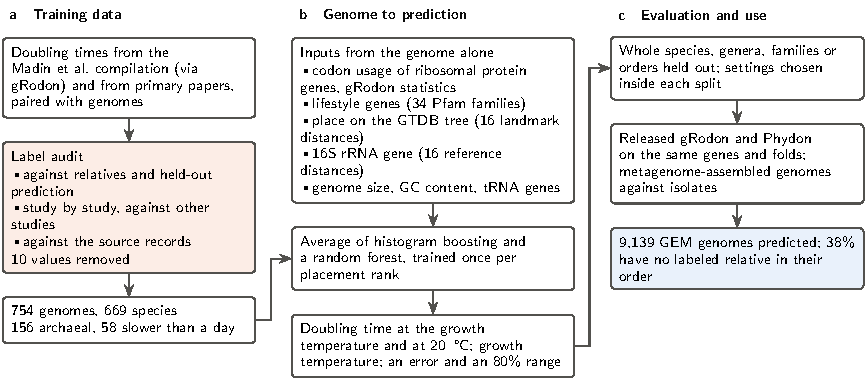
\includegraphics[width=0.82\textwidth,alt={Flow diagram in three columns. Training data: doubling times from the Madin compilation and primary papers, a label audit that removed values which are not maximal growth rates, and the final training set. Genome to prediction: inputs computed from the genome, a model averaging histogram boosting and a random forest, and three predicted quantities with errors and ranges. Evaluation and use: lineage-held-out evaluation, comparison with released tools and with metagenome-assembled genomes, and predictions for the GEM catalog.}]{fig1_overview_standalone}
\caption{Overview. (a) Growth rates were collected and audited for values that are not maximal growth rates. (b) Every input
is computed from the genome, so the same model applies to isolates and to metagenome-assembled genomes. (c) Accuracy is
measured with whole lineages held out, which is the situation of most environmental genomes, and the measured error at each
level of novelty is attached to every prediction.}
\label{fig:overview}
\end{figure*}
